\chapter{Orderbook Data}
\hrule
\vspace{40pt}

\section{Orderbook Mechanism}
On centralized exchanges, \textit{the orderbook} is the main data structure used to
organize buying and selling activity. 
There are two main orders a client can submit, \textit{market orders} and \textit{limit orders}.
Market orders get instantly matched at the \textit{best available price}
and executed. Limit orders specify a desired transaction price to buy/sell for a given volume.
If the order cannot be instantly filled by current supply, the limit order will
be posted to the limit orderbook, to be filled by future matching orders.
Essentially the orderbook keeps track of the current (unfilled) supply and demand.
The limit orders that are posted to the orderbook are organized into levels,
indexed by price. So all limit orders with the same price (and side) are 
combined into a single level, and their volumes are aggregated.
Note that the orderbook can contain hundreds of thousands of levels but the majority
of the activity is focused around the top levels.
The \textit{bids} are the buy orders, and the \textit{asks}
are the sell orders. Ask levels are sorted by price in ascending order and 
bid levels are sorted in descending order. The first/top ask level price is the
lowest ask price, and the first/top bid level price is the highest bid price. 
So if a client wishes to buy, the \textit{best available price} is the first/top/lowest ask price
and if they wish to sell, their best available price is first/top/highest bid price.
See Figure \ref{fig:orderbook} for a visual representation of the limit orderbook.
When new orders arrive, they will be matched against the orderbook and either posted or filled.
If enough orders are matched at a certain price, all the volume for that price level 
will be consumed and the price will be removed from the orderbook and the next best price will take its place for that level.
In this way, the state of the orderbook is constantly changing, as new orders are submitted
and price levels are partially or fully filled.

We define the mid-price to be the average of the best bid and ask price.
This single value is often used to represent the current price of the asset.
We also define the spread to be the difference between the best bid and ask price.
Smaller spreads are highly correlated with high trade volume \cite{ARITRA2021}.

\begin{figure}[htpb]
    \centering
    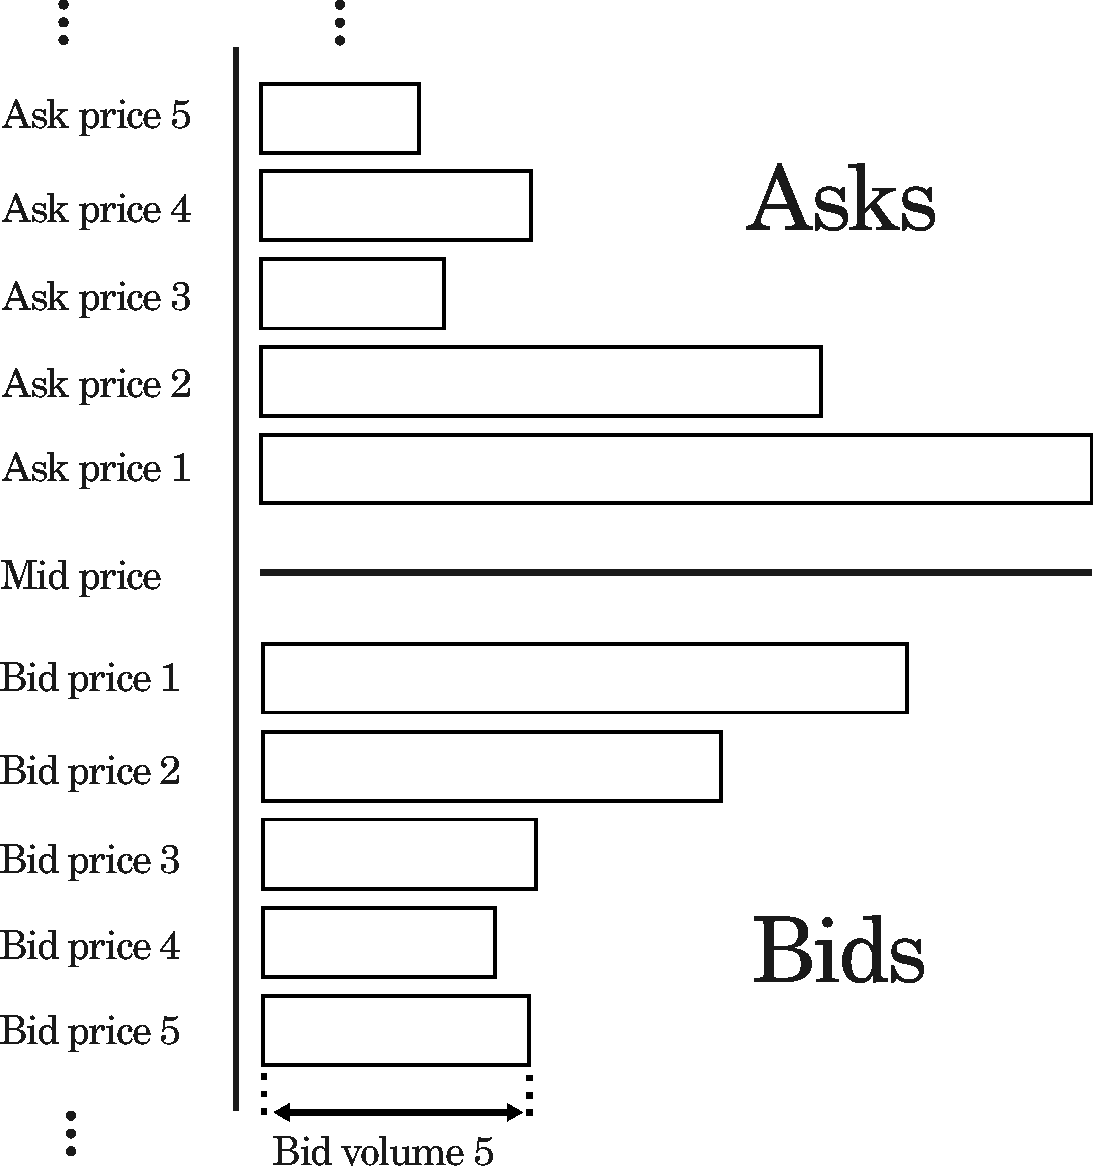
\includegraphics[width=0.5\textwidth]{./images/orderbook.pdf}
    \caption{A visual representation of the orderbook (specifically for L2 data).}
    \label{fig:orderbook}
\end{figure}

It is important to note that there are three main levels of granularity 
when it comes to orderbook representations.
Firstly we have L1 data, which is only the best bids and asks, with their corresponding volumes.
Then we have L2 data, which is all price levels with their corresponding volumes, with one volume value
per price level (i.e. volumes are summed across orders for each price level). Then the most granular is L3 data,
which contains all price levels, with multiple volume values for each price level. Specifically the volumes at a given price
level are broken down into their individual order values. So if, from time $t-1$ to time $t$, 2 orders
are submitted with volumes $v_a$ and $v_b$, then the $L2$ representation would show $V_t = V_{t-1} + v_a + v_b$,
whereas the L3 representation would give us  $\bm{V_t} = [\bm{V_{t-1}}; v_a, v_b]$

For a more in-depth exposition of the mechanism of the limit orderbook, we refer the interested reader to \cite{MARTIN2013}.


\section{The Data}
In this section we introduce our data source and give some visualizations.

\subsection{Data Source}

Our data has been gathered from Binance directly.
Binance is the largest cryptocurrency exchange in terms of daily volume, with a revenue of \$12 billion in 2022 according to \cite{TULLY2023}. 
It was founded in 2017 by Changpeng Zhao. %Binance was initially based in China, then moved to Japan shortly before the Chinese government restricted cryptocurrency companies. Binance then left Japan for Malta and currently has no official company headquarters. 
Binance was chosen because of its high volume, popularity and decent API availability.
Binance also offers perpetual USDT futures which is the main security of focus for this paper.

\subsection{Websocket Data}
Most communication on the internet takes place via a communication protocal known as HTTP, or 
Hypertext Transfer Protocol, \cite{HTTP1999}.
HTTP works in a single direction. We send a request to a server, then the server sends back a response
and then the connection is closed.
Of course for real time streaming applications this is too slow and ideally we would like to keep
the connection open continuously. Introducing the WebSocket protocol, \cite{WEBSOCKET2011}.
WebSocket is a bidirectional communication protocol that can send data from a client to a server
or from a server to a client by reusing the established connection channel.
The connection is kept open until terminated by either the server or the client.
Almost all live streaming applications such as trading, monitoring, etc. use the
WebSocket protocol to continuously receive the live data on a single communication channel.

Binance offers live Websocket data with various endpoints. 
We use the endpoint: 

\url{wss://fstream.binance.com/ws/{trading pair}@depth{L}@100ms}

to stream top L best bids and asks every approximately 100ms.
We log this data to an SQL database on an AWS server.
Due to free-tier limitations we only have about 30GB of storage on the server,
which corresponds to approximately a month of data for four trading pairs. 
This is also about the limit of how much data we can fit into memory at any one time. For these reasons
we only work with 20 days of data, from the start to the end of February, 2024. Specifically
we have data for 2024-02-05 13:07:53.664 until 2024-02-25 11:18:50.866.
This gives us approx. 12 million datapoints for each trading pair.
Since we are looking at such high frequencies, this data should be satisfactory.
We choose BTCUSDT, ETHUSDT, SOLUSDT and MATICUSDT as our futures trading pairs of interest. We choose
these because they are all high enough volume to have good liquidity but also have significant
enough difference in traded volume so that their comparative study should be interesting.
We store this data as a DataFrame for each trading pair. Each row contains the top 10 bid and ask prices and quantities
for a given time. See Table \ref{table:websocket} for an example DataFrame for MATICUSDT. 

\begin{table}[ht]
\centering
\resizebox{0.99\textwidth}{!}{
    \begin{tabular}{llllllllllllll}
    \toprule
    Row & timestamp & ask\_price\_1 & ... & ask\_price\_10 & bid\_price\_1 & ... & bid\_price\_10 & ask\_qty\_1 & ... & ask\_qty\_10 & bid\_qty\_1 & ... & bid\_qty\_10 \\
    \midrule
    0 & 1707138494390 & 0.7877 & ... & 0.7886 & 0.7876 & ... & 0.7867 & 9368.0 & ... & 58006.0 & 15095.0 & ... & 44990.0 \\
    1 & 1707138494515 & 0.7877 & ... & 0.7886 & 0.7876 & ... & 0.7867 & 9367.0 & ... & 58006.0 & 15095.0 & ... & 84785.0 \\
    2 & 1707138494760 & 0.7877 & ... & 0.7886 & 0.7876 & ... & 0.7867 & 9367.0 & ... & 58006.0 & 15095.0 & ... & 44990.0 \\
    3 & 1707138494881 & 0.7877 & ... & 0.7886 & 0.7876 & ... & 0.7867 & 9367.0 & ... & 58006.0 & 15095.0 & ... & 44990.0 \\
    4 & 1707138495248 & 0.7877 & ... & 0.7886 & 0.7876 & ... & 0.7867 & 9356.0 & ... & 58006.0 & 15099.0 & ... & 44990.0 \\
    \vdots & \vdots & \vdots & \vdots & \vdots & \vdots & \vdots & \vdots & \vdots & \vdots & \vdots & \vdots & \vdots & \vdots \\
    11294483 & 1708857980137 & 0.9726 & ... & 0.9735 & 0.9725 & ... & 0.9716 & 16199.0 & ... & 64495.0 & 20555.0 & ... & 37554.0 \\
    11294484 & 1708857980246 & 0.9726 & ... & 0.9735 & 0.9725 & ... & 0.9716 & 16199.0 & ... & 61163.0 & 19527.0 & ... & 37554.0 \\
    11294485 & 1708857980360 & 0.9726 & ... & 0.9735 & 0.9725 & ... & 0.9716 & 20199.0 & ... & 61163.0 & 19527.0 & ... & 37554.0 \\
    11294486 & 1708857980494 & 0.9726 & ... & 0.9735 & 0.9725 & ... & 0.9716 & 21610.0 & ... & 61163.0 & 19577.0 & ... & 37554.0 \\
    11294487 & 1708857980602 & 0.9726 & ... & 0.9735 & 0.9725 & ... & 0.9716 & 22992.0 & ... & 61163.0 & 18401.0 & ... & 37554.0 \\
    \bottomrule
    \end{tabular}
}
\caption{Example data for MATICUSDT.}
\label{table:websocket}
\end{table}

We note that the websocket data is not regular, but comes \textbf{approximately} every 100ms.
This means that the time difference/timedelta, $\Delta t$ ms between updates is not constant and therefore this is technically not
a timeseries in the proper sense. For some of our applications we will resample this data into regular intervals.
We present summary statistics for the timedeltas for each symbol in table \ref{timedelta_table}. We see that most of
the timedeltas are larger than the 100ms promised by the endpoint, with a mean of 133ms and median 116ms.
We also see a maximum timedelta of around 1 minute and a minimum timedelta of 3ms. Whilst this is less than
ideal for an experimental setup, we leave these outliers in, since they represent the real world inconsistencies that
one would find when using such a data source.

\begin{table}[ht]

\resizebox{\textwidth}{!}{
    \begin{tabular}{lrrrr}
    \toprule
     & BTCUSDT $\Delta t$ ms & ETHUSDT $\Delta t$ ms & MATICUSDT $\Delta t$ ms & SOLUSDT $\Delta t$ ms \\
    \midrule
    count & 12891080 & 13612890 & 11294487 & 13334051 \\
    median & 116 & 114 & 122 & 115 \\
    mean & 133 & 126 & 152 & 129 \\
    std & 50& 41& 82& 47\\
    min & 3 & 3 & 3 & 3 \\
    25\% & 107 & 105 & 108 & 107 \\
    50\% & 116 & 114 & 122 & 115 \\
    75\% & 142 & 133 & 162 & 135 \\
    max & 61604 & 61862 & 61697 & 61815 \\
    \bottomrule
    \end{tabular}
}

\caption{Summary statistics for the time difference between observations in our dataset in ms, $\Delta t$ ms, for each trading pair.}
\label{timedelta_table}
\end{table}

\begin{figure}[ht]
    \centering
    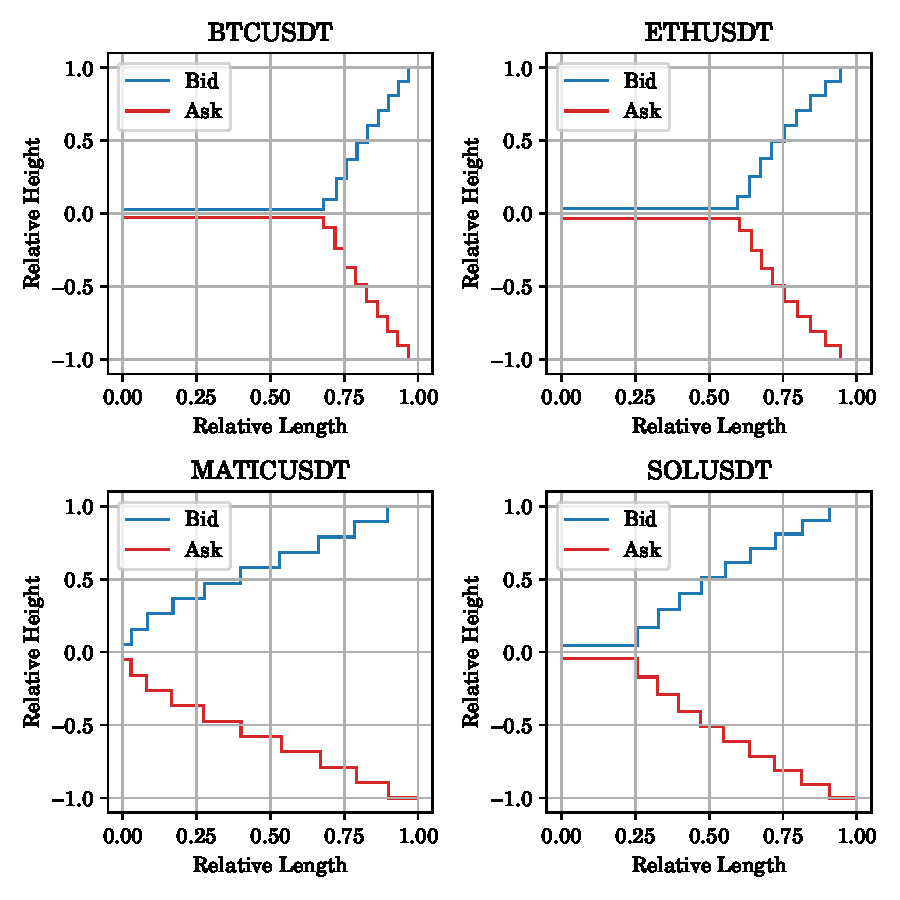
\includegraphics[width=0.99\textwidth]{./images/shapes.pdf}
    \caption{Average orderbook shape for each trading pair.}
    \label{shape}
\end{figure}

\clearpage

\section{Orderbook Shape}

In this section we aim to give a general overview of the shape of the orderbook for each trading pair in our data.
We define the height of a level $\ell \in \{ 1, 2, \dots, 10 \}$ on the $x$ side as $\Delta p_{\ell}^x = p_{\ell}^x - p_{\ell-1}^x$, with $x \in{\{ B,A \}}$. 
Where $B,A$ denote the bid, ask sides respectively. 
In other words, the price difference between the $\ell^{th}$ and $\ell-1^{th}$ bid/ask price level.
We note that by definition, $\Delta p_{\ell}^A < 0, ~ ~ \forall \ell$ and $\Delta p_{\ell}^B > 0, ~ ~ \forall \ell$.
The length of a level $\ell$ on the $x$ side is denoted by $q^x_{\ell}$ and represents the total volume
for the $\ell^{th}$ price level.
We also define the mid-price as an average of the best bid and ask price, i.e.
\begin{equation}
    p_0 := \frac{1}{2} (p^A_{1} + p^B_{1}) \label{mid}
\end{equation}
Following \cite{CAO2009}, we normalize the level heights by the price difference
between the 10th level and the mid-price, i.e. total height. 
The level length is also normalized by the total length from the first level to the 10th level, i.e.
\begin{align}
    \tilde{q}_{l}^x &:= \frac{q_{l}^x}{\sum_{j=1}^{10} q_{j}^x}  \\
    \Delta\tilde{p}_{l}^x &:= \frac{\Delta p_{l}^x}{\sum_{j=1}^{10} \Delta p_{j}^x} = \frac{\Delta p_{l}^x}{|p_{0} - p_{10}^x|}
\end{align}

We average the bids and asks over all entries and then calculate the normalized lengths
and heights. We visualize the results for each trading pair in Figure \ref{shape}.
This gives us a good idea of the overall average shape of the orderbooks.

We see that across all trading pairs the average orderbook is mostly symmetric,
which is what we would expect. Perhaps more interestingly we see that for BTCUSDT the relative
length for the first price level is much larger (higher volume) compared to the other top 10 levels.
In fact, we observe that the relative length of the first level seems to be increasing as a function
of the trading pairs popularity/volume. If we were to order the trading pairs in terms of trading volume, from 
lowest to highest we would have MATICUSDT, SOLUSDT, ETHUSDT and BTCUSDT. This ordering
is also the ordering of the relative length of the first level. So it seems that
the more popular a trading pair is, the more the volume is weighted towards the top of
the orderbook. Also another interesting point is that after the first level
the relative lengths are almost identical, suggesting e.g. that there is just as much
activity in the 10th level compared to the 2nd level of the orderbooks.
\cite{CAO2009} used a similar methodology to visualize the shape of the orderbook,
but for stocks from the Australian Securities Exchange, ASX. The shape of the orderbook
found in \cite{CAO2009} looks a lot like the MATICUSDT orderbook shape, which
agrees with our previously discussed first level length - volume relationship, since the ASX
(in 2009) had much less volume compared to BTCUSDT in 2024.

\section{Orderflow Imbalance}
In this section we introduce a key concept in this paper, \textit{orderflow}, which was first introduced in
\cite{CONT2013}, in the context of linear price impact modelling. We take a brief detour
here to apply this model to our data, in order to motivate the use of orderflow later on in our predictive modelling.

We start by defining the Orderflow Imbalance, a stationary transformation of the orderbook data
first introduced in \cite{CONT2013}.
Since mid-price movement is governed by supply and demand, we need to identify
the different orderbook states and how they relate to supply and demand.
We will initially only concern ourselves with the top of the orderbook.

For each of our observations, we have the best bid price and best bid quantity,
which we denote by $p^B, q^B$ and the best ask price and best ask quantity  $p^A, q^A$.
If we enumerate our observations through time by $n$, then according to \cite{CONT2013}, we have
the following orderbook events:
 \begin{itemize}
     \item $p_n^B > p_{n-1}^B$ or  $q_n^B > q_{n-1}^B$, suggesting an increase in demand.
     \item $p_n^B < p_{n-1}^B$ or  $q_n^B < q_{n-1}^B$, suggesting a decrease in demand.
     \item $p_n^A < p_{n-1}^A$ or  $q_n^A > q_{n-1}^A$, suggesting an increase in supply.
     \item $p_n^A > p_{n-1}^A$ or  $q_n^A < q_{n-1}^A$, suggesting a decrease in supply.
\end{itemize}
Then \cite{CONT2013} defines the quantity $e_n$ to represent the contribution of the  $n^{\text{th}}$ event
as $e_n := e_n^B - e_n^A$ where  $e_n^B$ and $e_n^A$ are defined in (\ref{eBeA}).
\begin{equation}
    \begin{aligned}
        e_{n}^B &:= I_{\{ p_{n}^B \geq p_{n-1}^B \}} q_{n}^B  - I_{\{ p_{n}^B \leq p_{n-1}^B \}} q_{n-1}^B \\
        e_{n}^A &:= I_{\{ p_{n}^A \leq p_{n-1}^A \}} q_{n}^A - I_{\{ p_{n}^A \geq p_{n-1}^A \}} q_{n-1}^A
    \end{aligned}
    \label{eBeA}
\end{equation}
% &= (\Delta q_{n}^B I_{\{ \Delta p_{n}^B \leq 0 \}} + q_{n}^B (I_{\{ \Delta p_{n}^B \geq 0 \}}  - I_{\{ \Delta p_{n}^B \leq 0 \}})) - (\Delta q_{n}^A I_{\{ \Delta p_{n}^A \geq 0 \}} + q_{n}^A (I_{\{ \Delta p_{n}^A \leq 0 \}} - I_{\{ \Delta p_{n}^A \geq 0\}})) \label{diff}
% Where (\ref{diff}) allows for efficient computation using the diff operator.
Then we sum these individual contributions from time $t-h$ to the current time $t$,
to get the Order Flow Imbalance at time $t$:
\begin{equation}
    \text{OFI}_h(t) := \sum_{n : t_n \in [t-h, t]} e_n
    \label{OFI}
\end{equation}

\subsection{Linear Price Impact Model}
In this subsection we introduce the linear price impact model from \cite{CONT2013} that motivates
the above orderflow definition.
Firstly, let us define $\Delta p_{\delta}(t+h) := (p(t+h) - p(t)) / \delta$, i.e. the change in price
measured in ticks, where $\delta$ is the ticksize for the given trading pair. Note that a tick
is defined as the smallest price increment in which the price for a pair is quoted, i.e. the precision.
Using the Binance API we
retrieve the ticksizes as:  % TODO: Format this better
\begin{table}[ht]
    \centering
    \begin{tabular}{ll}
        \toprule
        trading pair & $\delta$ \\
        \midrule
        BTCUSDT & 0.1 \\
        ETHUSDT & 0.01 \\
        SOLUSDT & 0.001 \\
        MATICUSDT & 0.0001 \\
        \bottomrule
    \end{tabular}
    \caption{Trading pairs and their ticksizes, $\delta$.}
\end{table}

\cite{CONT2013} considers a stylized model of the orderbook where the volume beyond the top level
is equal to $D$ and all trading activity only occurs at the top level. Of course this is a big
assumption but from our previous exploration we showed this to be largely justified for high volume pairs such
as BTCUSDT and ETHUSDT. Under these assumptions, we have three main events on the bid side:
\begin{enumerate}
    \item Market sell orders remove $M^s$ volume from the bid.
    \item Limit buy orders add $L^b$ volume to the bid.
    \item Limit buy cancels remove $C^b$ volume from the bid.
\end{enumerate}
We can analogously define quantities for the ask side.
Then under the above assumptions:
\begin{equation}
    \Delta p = \left\lceil (L^b - C^b - M^s) / 2D \right\rceil  - \left\lceil (L^s -C^s - M^b) / 2D \right\rceil
\end{equation}

This is equivalent, (up to some truncation) to:
\begin{equation}
    \Delta p = \frac{\text{OFI}}{2D} + \epsilon
\end{equation}
since $\text{OFI} = L^b - C^b-M^s-L^s+C^s+M^b$.

So under our stylized assumptions, we see that the price change in ticks
is directly proportional to the Orderflow Imbalance.
Therefore \cite{CONT2013} suggest the following relation:
\begin{equation}
    \Delta p_{\delta}(t) = \beta \text{OFI}_h(t) + \epsilon_t \label{linearrelation}
\end{equation}
where $\beta$ is the \textit{price impact coefficient} and $\epsilon_t$ is the noise
term. So $\beta$ measures the instantaneous impact of the $n^{th}$ event on the mid-price. 
\cite{CONT2013} assume the price impact coefficients are constant for half-hour intervals (indexed by $i$),
and estimate them using OLS:
\begin{equation}
    \Delta p_{\delta}(t) = \hat{\beta}_i \text{OFI}_h(t) + \hat{\alpha}_i + \hat{\epsilon}_t
\end{equation}

\subsection{PanelOLS Results}
We split our data into half-hour windows and then perform PanelOLS across windows
to estimate the average coefficients. We set $h = 1000ms$ and present the results for
BTCUSDT here. (The $R^2$ values for the other symbols are very similar and can be found in the appendix).

\begin{table}[H]
\textbf{BTCUSDT PanelOLS Results for h = 1000ms}
\begin{center}
\begin{tabular}{lclc}
\hline
\textbf{Dep. Variable:}    &         $\Delta p_{\delta}$         & \textbf{  R-squared:         }   &      0.3590      \\
\textbf{Estimator:}        &      PanelOLS      & \textbf{  R-squared (Between):}  &     -0.3865      \\
\textbf{No. Observations:} &      12891080      & \textbf{  R-squared (Within):}   &      0.3590      \\
\textbf{Date:}             &  Tue, Mar 26 2024  & \textbf{  R-squared (Overall):}  &      0.3585      \\
\textbf{Time:}             &      16:15:04      & \textbf{  Log-likelihood     }   &    -6.11e+07     \\
\textbf{Cov. Estimator:}   &     Clustered      & \textbf{                     }   &                  \\
\textbf{}                  &                    & \textbf{  F-statistic:       }   &    7.218e+06     \\
\textbf{Entities:}         &        956         & \textbf{  P-value            }   &      0.0000      \\
\textbf{Avg Obs:}          &     1.348e+04      & \textbf{  Distribution:      }   &  F(1,12890123)   \\
\textbf{Min Obs:}          &       953.00       & \textbf{                     }   &                  \\
\textbf{Max Obs:}          &     1.676e+04      & \textbf{  F-statistic (robust):} &      4743.2      \\
\textbf{}                  &                    & \textbf{  P-value            }   &      0.0000      \\
\textbf{Time periods:}     &       16761        & \textbf{  Distribution:      }   &  F(1,12890123)   \\
\textbf{Avg Obs:}          &       769.11       & \textbf{                     }   &                  \\
\textbf{Min Obs:}          &       1.0000       & \textbf{                     }   &                  \\
\textbf{Max Obs:}          &       956.00       & \textbf{                     }   &                  \\
\textbf{}                  &                    & \textbf{                     }   &                  \\
\hline
\end{tabular}
\begin{tabular}{lcccccc}
             & \textbf{Parameter} & \textbf{Std. Err.} & \textbf{T-stat} & \textbf{P-value} & \textbf{Lower CI} & \textbf{Upper CI}  \\
\hline
\textbf{OFI} &       1.1829       &       0.0172       &      68.871     &      0.0000      &       1.1492      &       1.2166       \\
\hline
\end{tabular}
%\caption{PanelOLS Estimation Summary}
\end{center}
F-test for Poolability: 19.309, \\
Distribution: F(955,12890123),\\
Included effects: Entity.
\end{table}

\begin{figure}[H]
    \centering
    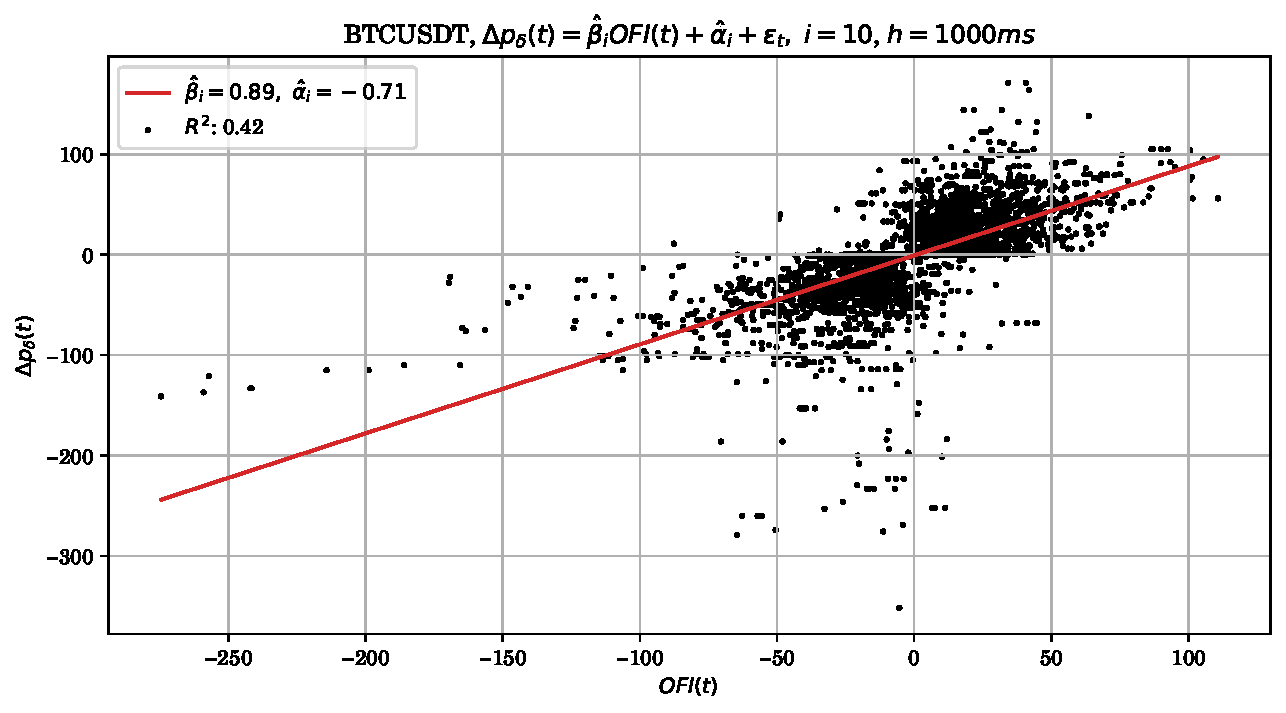
\includegraphics[width=0.8\textwidth]{./images/btcusdt_h=1000ms_contemp_OFI.pdf}
    \caption{OFI contemporaneous regression for an example half-hour window for BTCUSDT.}
    \label{fig:contemp_OFI_btcusdt}
\end{figure}

We observe very similar $R^2$ values across all trading pairs, around $0.35$, confirming the
linear relation (\ref{linearrelation}). We also visualize the regression for an example half hour window in Figure \ref{fig:contemp_OFI_btcusdt}.
% Interestingly we see that the $\Delta p_{\delta}(t)$ values for MATICUSDT
% are far more sparse than the other trading pairs, with fewer unique values, and much more clearly
% defined steps. This is much more similar to the results of \cite{CONT2013} and 
% perhaps is characteristic of securities with lower volume.

We repeat the procedure for different values of $h$ and plot the results in Figure \ref{r2_h}.
We see that $R^2$ increases in  $h$ and then plateaus around $h=20,000ms$.

Instead of averaging across intervals, we can also examine how the price impact coefficients change
across intervals. We visualize the results in Figures \ref{fig:BTCUSDT_beta_across_time} - \ref{fig:MATICUSDT_beta_across_time}.
We see that, for our data, for all trading pairs the average price impact coefficient is initially decreasing in time
for the first few hours of the day. It then recovers and begins to (roughly) increase again.
We also see that the variance of the price impact coefficients are fairly constant across different intervals.
The fact that we have trends in price impact coefficients suggests that
the impact of a new orderbook event on the mid-price varies throughout the day, with
some periods having less impact (assuming the linear price impact model given by (\ref{linearrelation})).
The smallest average coefficients seem to occur around 06:00AM and so we suggest placing trades around this time
if the goal is to minimize price impact.

\subsection{Conclusion}
Whether this model is too simple to realistically model price impact in a useful way is not something we explore in this paper.
The purpose of this section rather, was to introduce orderflow and show that it has relevance for influencing price changes in the orderbook.


\begin{figure*}[htpb]
   \centering
   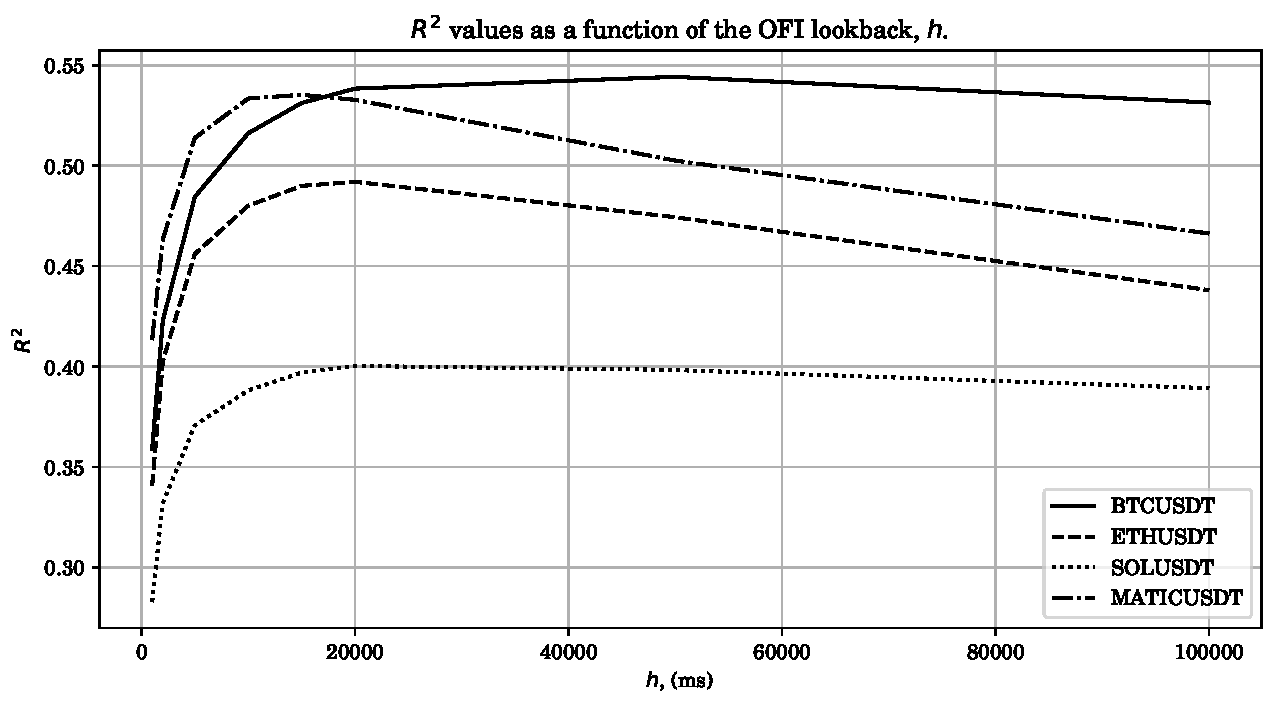
\includegraphics[width=1.0\textwidth]{./images/OFI_r2_h.pdf}
   \caption{Effect on contemporaneous regression $\Delta p_{\delta}(t) = \hat{\beta}_i \text{OFI}_h(t) + \hat{\alpha}_i + \hat{\epsilon}_t$,
       $R^2$ values when varying the lookback period, $h$, that defines $\text{OFI}_h(t)$.
    }
   \label{r2_h}
\end{figure*}

\clearpage

\begin{figure*}[htpb]
    \centering
    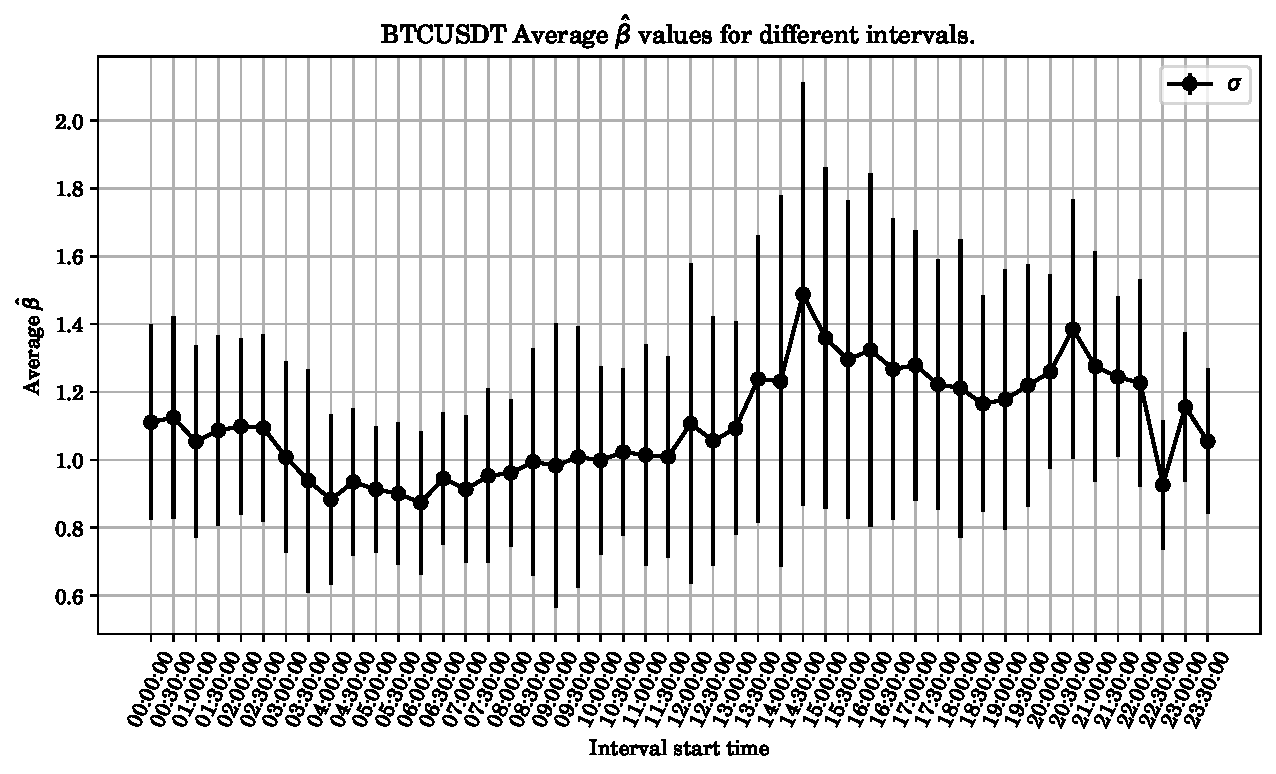
\includegraphics[width=0.8\textwidth]{./images/BTCUSDT_beta_across_time.pdf}
    \caption{BTCUSDT Average price impact coefficients for different half-hour intervals. Note that errorbars represent standard deviations.}
    \label{fig:BTCUSDT_beta_across_time}
\end{figure*}


\begin{figure*}[htpb]
    \centering
    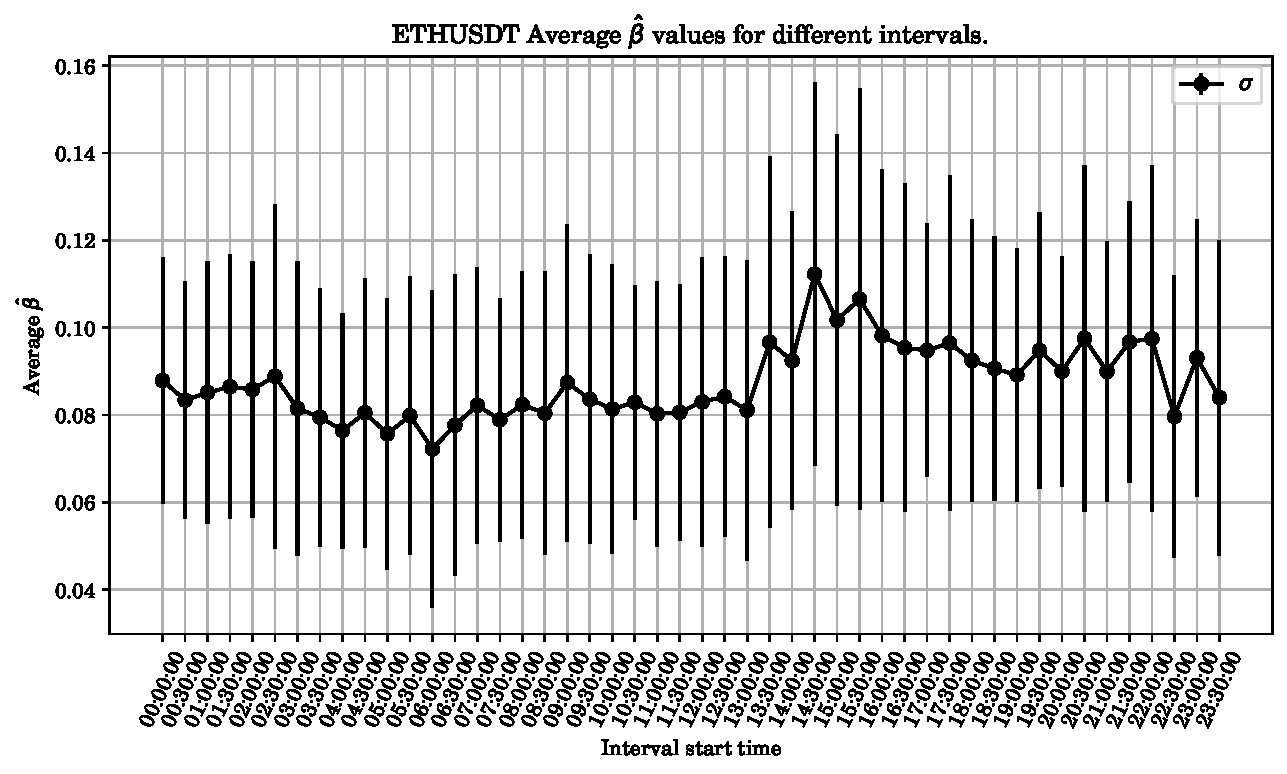
\includegraphics[width=0.8\textwidth]{./images/ETHUSDT_beta_across_time.pdf}
    \caption{ETHUSDT Average price impact coefficients for different half-hour intervals. Note that errorbars represent standard deviations.}
\end{figure*}

\begin{figure*}[htpb]
    \centering
    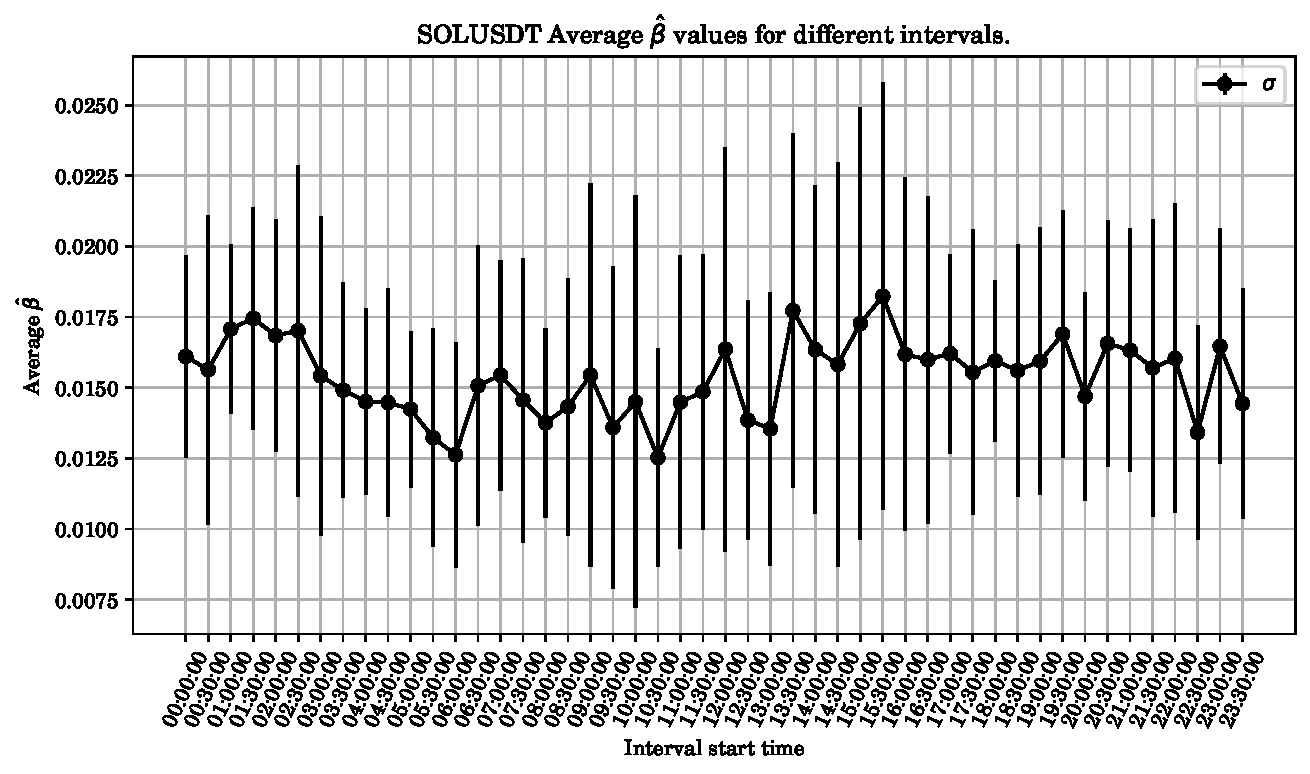
\includegraphics[width=0.8\textwidth]{./images/SOLUSDT_beta_across_time.pdf}
    \caption{SOLUSDT Average price impact coefficients for different half-hour intervals. Note that errorbars represent standard deviations.}
\end{figure*}

\begin{figure*}[htpb]
    \centering
    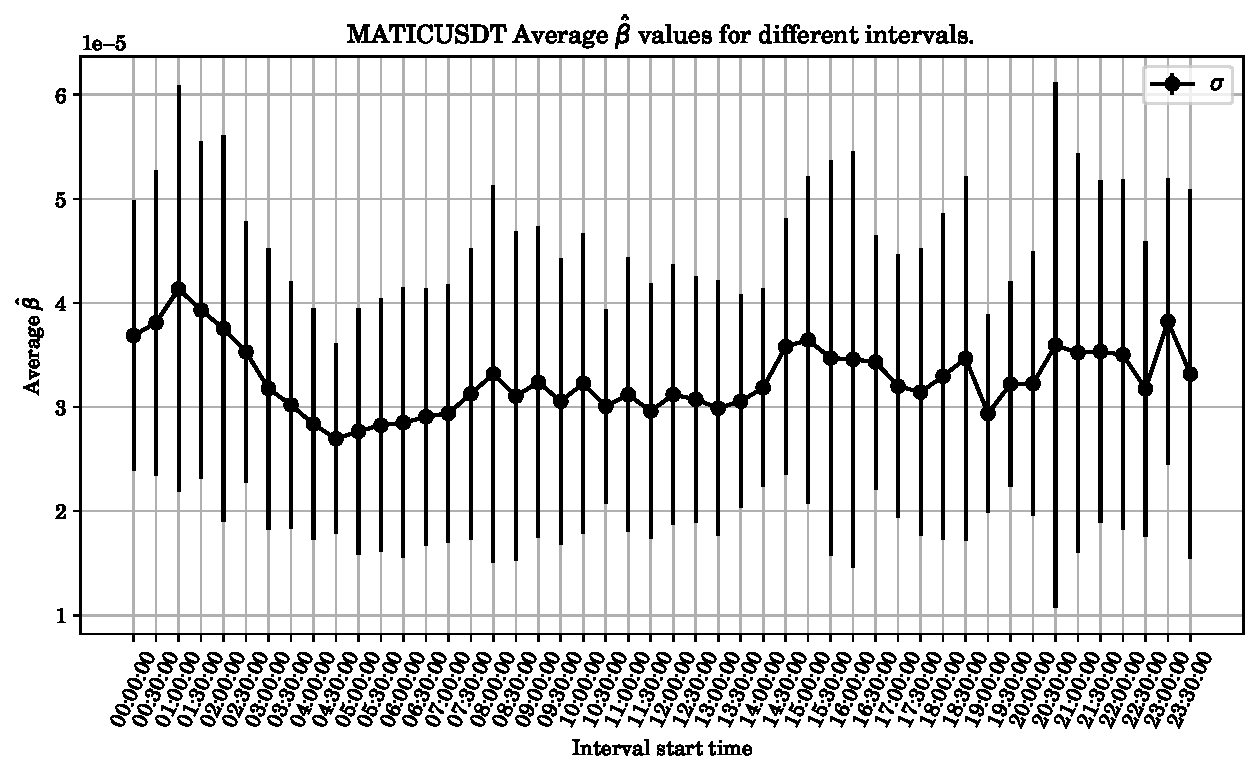
\includegraphics[width=0.8\textwidth]{./images/MATICUSDT_beta_across_time.pdf}
    \caption{MATICUSDT Average price impact coefficients for different half-hour intervals. Note that errorbars represent standard deviations.}
    \label{fig:MATICUSDT_beta_across_time}
\end{figure*}


